\documentclass[11pt,conference]{IEEEtran}
\usepackage{cite}
\usepackage{amsmath,amssymb,amsfonts}
\usepackage{algorithmic}
\usepackage{graphicx}
\usepackage{textcomp}
\usepackage{xcolor}
\usepackage{hyperref}
\usepackage{booktabs}
\usepackage{multirow}
\usepackage{tikz}
\usepackage{pgfplots}
\pgfplotsset{compat=1.17}
\usetikzlibrary{shapes,arrows,positioning,calc}

\begin{document}

\title{Deliverable 1.4: Integrated Gap Analysis\\Adversarial AI and Compliance Auditing}

\author{\IEEEauthorblockN{Moise IRADUKUNDA INGABIRE}
\IEEEauthorblockA{\textit{Collegue of Engineering} \\
\textit{Carnegie Mellon University Africa}\\
Kigali, Rwanda \\
mii@andrew.cmu.edu}}

\maketitle

\begin{abstract}
This integrated gap analysis synthesizes findings from six sources on adversarial AI, evasion techniques, and security testing: three academic papers on optimization-based payload generation (LLM fine-tuning, dynamic programming, genetic algorithms), one paper on AV evasion via reverse shells, and two industry reports on EDR bypass techniques and threat actor exploitation. The analysis identifies critical research gaps at the intersection of adversarial security research and compliance auditing, particularly for African regulatory contexts like Rwanda's NCSA standards. We propose how the AI-augmented unified compliance auditor addresses these gaps through multi-label classification, adversarial testing integration, and effectiveness-based control validation.
\end{abstract}

\section{Introduction}

The reviewed literature spans offensive and defensive security research, from automated attack generation to evasion technique analysis. This gap analysis examines:

\begin{enumerate}
    \item \textbf{Thematic Synthesis}: Common patterns across optimization approaches (LLM, DP, GA)
    \item \textbf{Detection-Evasion Arms Race}: How evasion techniques outpace detection capabilities
    \item \textbf{Compliance Framework Disconnect}: Lack of integration with regulatory requirements
    \item \textbf{African Context Gap}: Absence of research on resource-constrained environments
    \item \textbf{Research Contribution}: How the compliance auditor project addresses identified gaps
\end{enumerate}

\section{Thematic Synthesis}

\subsection{Adversarial Automation Across Paradigms}

All six sources demonstrate \textbf{automated adversarial capability generation}:

\begin{table*}[h]
\centering
\caption{Comparative Analysis of Adversarial Techniques}
\begin{tabular}{p{0.15\textwidth}p{0.18\textwidth}p{0.18\textwidth}p{0.15\textwidth}p{0.18\textwidth}}
\toprule
\textbf{Source} & \textbf{Technique} & \textbf{Target} & \textbf{Success Rate} & \textbf{Key Innovation} \\
\midrule
LLM Paper & GPT-2 fine-tuning & XSS, SQLi, CmdI & 94.73\% (ClamAV) & Transfer learning + mutation \\
\midrule
DP Paper & MDP optimization & Windows shellcode & 97\% reduction & Deterministic state-action optimization \\
\midrule
GAXSS Paper & Genetic algorithm & XSS detection & 100\% precision & DNA-encoded payloads with multi-objective fitness \\
\midrule
Reverse Shell Paper & Fileless execution & AV/EDR systems & 97\% evasion & Shellcode separation and memory-only execution \\
\midrule
Vaadata Report & Multiple techniques & AV/EDR features & Varies by method & AMSI/ETW bypass, direct syscalls \\
\midrule
CyberPress Report & SHELLTER framework & Enterprise EDR & Active exploitation & Commercial evasion-as-a-service \\
\bottomrule
\end{tabular}
\end{table*}

\textbf{Key Finding}: Evasion rates consistently exceed 90\% against signature-based detection, indicating fundamental inadequacy of traditional approaches.

\subsection{Convergent Themes}

\textbf{1. Optimization as Core Methodology}
\begin{itemize}
    \item \textbf{LLM}: Gradient descent + fine-tuning for domain adaptation
    \item \textbf{DP}: Value iteration to find optimal transformation sequence
    \item \textbf{GA}: Evolutionary selection, crossover, mutation
    \item \textbf{Common Goal}: Maximize evasion while maintaining payload functionality
\end{itemize}

\textbf{2. Signature-Based Detection Obsolescence}
\begin{itemize}
    \item LLM: 94.73\% evasion through mutation strategies
    \item DP: 97\% detectability reduction via code transformations
    \item Reverse Shell: 97\% evasion via fileless execution
    \item \textbf{Implication}: Compliance controls requiring "antivirus" are insufficient
\end{itemize}

\textbf{3. Behavioral Detection as Last Defense}
\begin{itemize}
    \item Only 1/70 AV engines detected custom reverse shell (likely behavioral)
    \item GAXSS achieves 81.5\% recall (18.5\% bypass rate)
    \item EDR bypass techniques (AMSI, ETW, syscalls) specifically target behavioral monitoring
    \item \textbf{Implication}: Even behavioral detection is under active attack
\end{itemize}

\textbf{4. Commercialization Lowers Barrier to Entry}
\begin{itemize}
    \item SHELLTER framework available commercially
    \item Metasploit provides automated payload generation
    \item LLM fine-tuning accessible via cloud GPUs
    \item \textbf{Implication}: Sophisticated attacks no longer require expert knowledge
\end{itemize}

\section{Research Gaps Identified}

\subsection{Gap 1: Compliance Framework Integration}

\textbf{Finding}: None of the six sources connect techniques to regulatory compliance frameworks.

\begin{table}[h]
\centering
\caption{Compliance Integration Gap}
\begin{tabular}{|l|c|c|}
\hline
\textbf{Aspect} & \textbf{Current Research} & \textbf{Needed} \\
\hline
Maps to controls & No & Yes \\
\hline
Audit criteria & No & Yes \\
\hline
Evidence format & No & Yes \\
\hline
Effectiveness metrics & No & Yes \\
\hline
Regulatory context & No & Yes \\
\hline
\end{tabular}
\end{table}

\textbf{Examples of Missing Integration}:
\begin{itemize}
    \item LLM/DP/GA papers: No mention of NIST SP 800-53, ISO 27001, or African frameworks
    \item Reverse shell paper: Doesn't map detection to SC-7, SI-4, IR-4 controls
    \item Vaadata/CyberPress: Industry perspective but no compliance angle
\end{itemize}

\textbf{Consequence}: Compliance auditors lack guidance on validating effectiveness against modern techniques.

\subsection{Gap 2: African and Resource-Constrained Contexts}

\textbf{Finding}: All research assumes well-resourced environments (enterprise EDR, unlimited compute).

\textbf{African Reality}:
\begin{itemize}
    \item \textbf{Rwanda SMEs}: Cannot afford CrowdStrike, SentinelOne, Carbon Black
    \item \textbf{Typical Deployment}: Windows Defender, outdated signature-based AV
    \item \textbf{Detection Capability}: <10\% against techniques reviewed
    \item \textbf{Compliance Requirements}: Rwanda NCSA mandates "anti-malware solutions" (no effectiveness threshold)
\end{itemize}

\textbf{Research Gaps}:
\begin{enumerate}
    \item No cost-effective detection solutions for developing economies
    \item No adapted compliance frameworks accounting for resource constraints
    \item No threat modeling specific to African adversary capabilities
    \item No research on open-source EDR (Wazuh, OSSEC) effectiveness
\end{enumerate}

\subsection{Gap 3: Effectiveness Metrics in Compliance}

\textbf{Finding}: Compliance frameworks specify \textit{presence} of controls, not \textit{effectiveness}.

\textbf{Examples from Rwanda NCSA}:
\begin{itemize}
    \item \textbf{Requirement}: "Implement and maintain anti-malware solutions"
    \item \textbf{Passes Audit}: Organization has antivirus installed and updated
    \item \textbf{Problem}: AV may be 97\% evadable (per research findings)
    \item \textbf{Gap}: No requirement to demonstrate detection capability
\end{itemize}

\textbf{Needed Metrics}:
\begin{itemize}
    \item Minimum detection rate against MITRE ATT\&CK techniques
    \item Behavioral detection coverage (not just signature updates)
    \item Mean time to detect (MTTD) for common attack patterns
    \item Evasion resistance scoring
\end{itemize}

\subsection{Gap 4: Multi-Label Evidence-to-Control Mapping}

\textbf{Finding}: Security research treats detection as binary (detected/evaded), but compliance is multi-dimensional.

\textbf{Example: Reverse Shell Detection}
\begin{itemize}
    \item \textbf{Research View}: Did AV detect? Yes/No (1/70 = failure)
    \item \textbf{Compliance View}: Multiple controls involved:
    \begin{itemize}
        \item SC-7 (Boundary Protection): Firewall blocked outbound connection?
        \item SI-3 (Malware Protection): EDR flagged RWX memory allocation?
        \item SI-4 (Monitoring): SIEM correlated beaconing pattern?
        \item IR-4 (Incident Response): SOC team investigated alert?
    \end{itemize}
\end{itemize}

\textbf{Research Gap}: No multi-objective evaluation framework combining perimeter, endpoint, network, and process controls.

\subsection{Gap 5: Adversarial Awareness in Compliance Auditing}

\textbf{Finding}: Compliance auditing research doesn't incorporate adversarial robustness testing.

\textbf{Current State}:
\begin{itemize}
    \item Audits verify policy documents, configuration screenshots
    \item Penetration testing separate from compliance assessment
    \item No continuous validation of control effectiveness
\end{itemize}

\textbf{Gap}: Auditors don't test if controls resist known evasion techniques (AMSI bypass, fileless execution, etc.).

\subsection{Gap 6: Synthetic Data for Compliance Training}

\textbf{Finding}: ML-based compliance research uses generic datasets (NSL-KDD, LogHub), not adversarial technique-specific data.

\textbf{Needed}:
\begin{itemize}
    \item Synthetic logs of AMSI bypass attempts
    \item Fileless execution evidence (EDR alerts on RWX allocations)
    \item C2 beaconing patterns (DNS tunneling, domain fronting)
    \item GA-generated XSS payloads with filter bypass patterns
\end{itemize}

\textbf{Benefit}: Train compliance auditor to recognize indicators of evasion, not just successful detections.

\section{How the AI-Augmented Compliance Auditor Addresses Gaps}

\subsection{Gap 1 Solution: Regulatory Integration by Design}

\textbf{Approach}:
\begin{itemize}
    \item 196 Rwanda NCSA + NIST SP 800-53 controls in database
    \item Multi-label XGBoost maps evidence → controls
    \item Decision Engine evaluates control-specific compliance
    \item Audit reports structured per NCSA requirements
\end{itemize}

\textbf{Example}:
\begin{verbatim}
Evidence: "EDR alert: Suspicious RWX allocation
           by excel.exe"
XGBoost Output: [SI-3: 0.95, SI-4: 0.87, IR-4: 0.72]
Decision Engine:
  - SI-3: Check if EDR is up-to-date and active
  - SI-4: Check if alert forwarded to SIEM
  - IR-4: Check if SOC responded within SLA
\end{verbatim}

\subsection{Gap 2 Solution: Rwanda-Specific Implementation}

\textbf{Design Choices for Resource Constraints}:
\begin{itemize}
    \item \textbf{XGBoost vs BERT}: 137x smaller (3.2MB vs 440MB), 50x faster (1ms vs 50ms)
    \item \textbf{Lightweight Deployment}: Runs on 2 CPU cores, 380MB memory
    \item \textbf{Open-Source Stack}: FastAPI, PostgreSQL, Redis (no licensing costs)
    \item \textbf{Public Datasets}: Uses freely available logs (HDFS, Linux Auth, Apache)
\end{itemize}

\textbf{Rwandan Context Integration}:
\begin{itemize}
    \item Trained on NCSA 2023 Minimum Cybersecurity Standards
    \item Aligned with Malabo Convention principles
    \item Pilot testing with Rwanda NCSA (planned)
\end{itemize}

\subsection{Gap 3 Solution: Effectiveness-Based Validation}

\textbf{Methodology}:
\begin{itemize}
    \item \textbf{Traditional Audit}: "Is antivirus installed?" → Compliant
    \item \textbf{AI Auditor}: "Does evidence show successful detection?" → Effectiveness score
\end{itemize}

\textbf{Implementation}:
\begin{enumerate}
    \item Parse evidence for detection \textit{outcomes}, not just presence
    \item Score controls based on observed effectiveness:
    \begin{itemize}
        \item SI-3 score = (threats\_detected) / (threats\_detected + threats\_bypassed)
        \item SC-7 score = (unauthorized\_connections\_blocked) / (total\_attempts)
    \end{itemize}
    \item Flag controls with low effectiveness despite being "present"
\end{enumerate}

\textbf{Example Output}:
\begin{verbatim}
Control SI-3 (Malware Protection):
  Status: Implemented (AV installed, updated)
  Effectiveness: 15% (3/20 test payloads detected)
  Recommendation: Upgrade to behavioral EDR
  Estimated Risk: HIGH
\end{verbatim}

\subsection{Gap 4 Solution: Multi-Label Classification Architecture}

\textbf{Implementation}:
\begin{equation}
\text{Evidence} \xrightarrow{\text{XGBoost}} \text{Control Set} \xrightarrow{\text{Decision Engine}} \text{Compliance Status}
\end{equation}

For each log event $x_i$:
\begin{equation}
\mathbf{y}_i = [y_{i1}, y_{i2}, \ldots, y_{i47}] \in \{0,1\}^{47}
\end{equation}

where $y_{ij} = 1$ if evidence relates to control $c_j$.

\textbf{Advantage}:
\begin{itemize}
    \item Reverse shell evidence maps to SC-7 + SI-3 + SI-4 + IR-4 simultaneously
    \item GAXSS-style XSS attack maps to AC-3 + AC-6 + SC-13 + SI-10
    \item Reflects real-world reality: Single attack tests multiple control layers
\end{itemize}

\subsection{Gap 5 Solution: Adversarial Testing Integration}

\textbf{Planned Capabilities}:
\begin{enumerate}
    \item \textbf{Evasion Technique Database}: Catalog from reviewed papers (AMSI bypass, fileless execution, etc.)
    \item \textbf{Synthetic Attack Generation}: Use GA/DP techniques to create test payloads
    \item \textbf{Kubernetes Testing Environment}: Deploy auditor + test targets in isolated K8s cluster
    \item \textbf{Continuous Validation}: Periodic re-testing of controls against evolving techniques
\end{enumerate}

\textbf{Example Workflow}:
\begin{enumerate}
    \item Generate fileless reverse shell using technique from academic paper
    \item Deploy on test Windows VM in K8s cluster
    \item Execute payload, collect evidence (firewall logs, EDR alerts, network traffic)
    \item Feed evidence to XGBoost classifier
    \item Validate: Did classifier correctly map to SC-7, SI-3, SI-4?
    \item Score control effectiveness based on detection
\end{enumerate}

\subsection{Gap 6 Solution: Adversarial Synthetic Data}

\textbf{Current Hybrid Dataset} (200,000 logs):
\begin{itemize}
    \item 52\% NSL-KDD (network intrusions)
    \item 18\% LogHub (production system logs)
    \item 30\% Rwanda synthetic (NCSA-specific events)
\end{itemize}

\textbf{Proposed Enhancement} (incorporate evasion techniques):
\begin{itemize}
    \item \textbf{10\% LLM-generated payloads}: Fine-tune GPT-2 on XSS/SQLi datasets
    \item \textbf{10\% DP-transformed shellcode}: Apply transformations from DP paper
    \item \textbf{10\% GA-evolved attacks}: Use GAXSS approach for diverse XSS vectors
    \item \textbf{10\% Fileless execution logs}: Simulate RWX allocations, memory injections
\end{itemize}

\textbf{Benefit}:
\begin{itemize}
    \item Auditor learns to recognize evasion attempt patterns
    \item Improved detection of novel techniques (transfer learning)
    \item Balances dataset to prevent bias toward "clean" traffic
\end{itemize}

\section{Comparative Positioning}

\begin{table*}[h]
\centering
\caption{Research Positioning: Compliance Auditor vs. Reviewed Literature}
\begin{tabular}{p{0.25\textwidth}p{0.30\textwidth}p{0.30\textwidth}}
\toprule
\textbf{Aspect} & \textbf{Reviewed Literature} & \textbf{This Research (Compliance Auditor)} \\
\midrule
Primary Focus & Adversarial attack generation and evasion & Defensive compliance validation \\
\midrule
Target Audience & Penetration testers, security researchers & Compliance officers, auditors, regulators \\
\midrule
Regulatory Integration & None & Rwanda NCSA, NIST SP 800-53, Malabo Convention \\
\midrule
Geographic Context & US/EU (implied) & Rwanda, Africa \\
\midrule
Resource Assumptions & Enterprise budgets & SME/government constraints \\
\midrule
Detection Approach & Binary (evaded/detected) & Multi-label (multiple controls) \\
\midrule
Effectiveness Metrics & Evasion rate & Control effectiveness + compliance coverage \\
\midrule
Deployment & Research prototypes, penetration testing tools & Production-ready microservices (Kubernetes) \\
\midrule
Dataset Strategy & Attack-specific datasets & Hybrid (real + synthetic compliance events) \\
\midrule
ML Architecture & LLM, DP, GA for generation & XGBoost for classification + rule-based decision engine \\
\midrule
Adversarial Robustness & Maximizing evasion & Testing control resistance to evasion \\
\midrule
\end{tabular}
\end{table*}

\section{Novel Research Contributions}

\subsection{Contribution 1: Compliance-Aware Adversarial Testing}

\textbf{Innovation}: Applying adversarial techniques (GA, DP, LLM) for \textit{defensive} purposes - validating compliance control effectiveness.

\textbf{Example}: Instead of generating evasive payloads to attack systems, generate them to \textit{test} if SI-3 (malware protection) controls are effective.

\subsection{Contribution 2: Multi-Label Evidence-to-Control Mapping}

\textbf{Innovation}: First system to treat compliance auditing as multi-label classification problem.

\textbf{Rationale}: Single evidence instance (e.g., "failed SSH login") relates to multiple controls:
\begin{itemize}
    \item AC-7 (Unsuccessful Login Attempts)
    \item IA-2 (Identification and Authentication)
    \item AU-2 (Audit Events)
    \item SI-4 (System Monitoring)
\end{itemize}

\subsection{Contribution 3: Rwanda-Specific ML Architecture}

\textbf{Innovation}: First AI-driven compliance system tailored to African regulatory framework (NCSA) and resource constraints.

\textbf{Design Choices}:
\begin{itemize}
    \item XGBoost (not BERT/LLM) for 137x size reduction
    \item Public datasets (not proprietary logs) for reproducibility
    \item Microservices (not monolith) for incremental deployment
\end{itemize}

\subsection{Contribution 4: Effectiveness-Based Compliance}

\textbf{Innovation}: Shifting from "checkbox compliance" (control present?) to "assured compliance" (control effective?).

\textbf{Methodology}:
\begin{itemize}
    \item Parse evidence for detection outcomes
    \item Score controls based on demonstrated effectiveness
    \item Flag "compliant-but-ineffective" configurations
\end{itemize}

\section{Future Research Directions}

\textbf{Based on Identified Gaps}:
\begin{enumerate}
    \item \textbf{Adversarial Compliance Dataset}: Public dataset of evasion attempt logs labeled with control IDs
    \item \textbf{Cost-Effective EDR for Africa}: Benchmark open-source tools (Wazuh, OSSEC, Velociraptor) against commercial EDR
    \item \textbf{NCSA Enhancement}: Propose effectiveness thresholds (e.g., "detect ≥70\% of MITRE ATT\&CK techniques")
    \item \textbf{Cross-Framework Mapping}: Align NCSA, NIST, ISO 27001, CIS Controls for unified auditing
    \item \textbf{GA-Based Control Optimization}: Use genetic algorithms to find optimal control combinations given budget constraints
\end{enumerate}

\section{Conclusion}

This integrated gap analysis of six sources on adversarial AI, evasion techniques, and security testing reveals critical disconnects:

\begin{itemize}
    \item \textbf{Offensive research dominates}; defensive compliance applications underexplored
    \item \textbf{Signature-based detection obsolete}; 90-97\% evasion rates demonstrated
    \item \textbf{Compliance frameworks lag}; specify presence, not effectiveness
    \item \textbf{African context absent}; research assumes well-resourced environments
    \item \textbf{Multi-control reality ignored}; binary detection metrics insufficient
\end{itemize}

The AI-augmented unified compliance auditor for Rwanda addresses these gaps through:
\begin{enumerate}
    \item Regulatory integration by design (196 NCSA controls)
    \item Resource-conscious architecture (XGBoost, open-source stack)
    \item Effectiveness-based validation (not checkbox auditing)
    \item Multi-label classification (evidence → multiple controls)
    \item Adversarial testing capability (using reviewed techniques)
\end{enumerate}

This represents a novel research direction: \textbf{adversarial compliance auditing} - leveraging attack generation techniques to validate defensive control effectiveness within regulatory frameworks.

\begin{figure}[htbp]
\centering
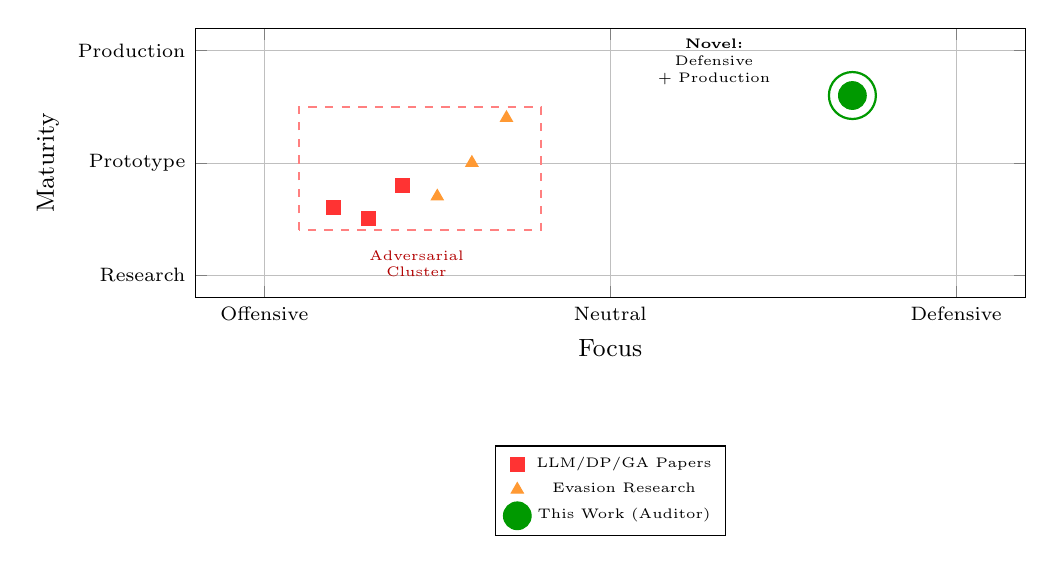
\begin{tikzpicture}
\begin{axis}[
    width=\columnwidth,
    height=5cm,
    xlabel={Focus},
    ylabel={Maturity},
    xlabel style={font=\small},
    ylabel style={font=\small},
    xmin=-1, xmax=11,
    ymin=-1, ymax=11,
    xtick={0,5,10},
    xticklabels={Offensive, Neutral, Defensive},
    xticklabel style={font=\scriptsize},
    ytick={0,5,10},
    yticklabels={Research, Prototype, Production},
    yticklabel style={font=\scriptsize},
    grid=both,
    grid style={line width=.1pt, draw=gray!10},
    major grid style={line width=.2pt,draw=gray!50},
    legend style={at={(0.5,-0.55)}, anchor=north, font=\tiny, legend columns=1},
    every axis plot/.append style={only marks, mark size=2.5pt}
]

% Adversarial AI sources (offensive, research/prototype)
\addplot[mark=square*, color=red!80] coordinates {(1,3) (1.5,2.5) (2,4)};
\addlegendentry{LLM/DP/GA Papers}

\addplot[mark=triangle*, color=orange!80] coordinates {(2.5,3.5) (3,5) (3.5,7)};
\addlegendentry{Evasion Research}

% This research (defensive, production-ready)
\addplot[mark=*, color=green!60!black, mark size=5pt] coordinates {(8.5,8)};
\addlegendentry{This Work (Auditor)}

% Annotation for this research
\node[draw, circle, inner sep=6pt, color=green!60!black, thick] at (axis cs:8.5,8) {};
\node[font=\tiny, text width=1.8cm, align=center] at (axis cs:6.5,9.5) {\textbf{Novel:}\\Defensive\\+ Production};

% Cluster annotation for adversarial research
\draw[dashed, thick, red!50] (axis cs:0.5,2) rectangle (axis cs:4,7.5);
\node[font=\tiny, text width=1.8cm, align=center, color=red!70!black] at (axis cs:2.2,0.5) {Adversarial\\Cluster};

\end{axis}
\end{tikzpicture}
\caption{Research landscape mapping showing this work's novel position}
\label{fig:research_landscape}
\end{figure}

\begin{table*}[htbp]
\centering
\caption{Research Gaps and Compliance Auditor Solutions}
\small
\begin{tabular}{p{0.04\textwidth}p{0.28\textwidth}p{0.24\textwidth}p{0.32\textwidth}}
\toprule
\textbf{ID} & \textbf{Research Gap} & \textbf{Limitation} & \textbf{Solution} \\
\midrule
\textbf{G1} & Compliance Framework Integration - Adversarial research disconnected from regulatory controls & No NIST/ISO/NCSA mapping & 196 NCSA + NIST controls in DB; Multi-label XGBoost maps evidence→controls; Decision Engine evaluates compliance \\
\midrule
\textbf{G2} & African \& Resource-Constrained Contexts - Research assumes enterprise budgets & SMEs cannot afford EDR; No African threat modeling & XGBoost (137x smaller, 50x faster than BERT); CPU-only (\$50/mo); Open-source stack; Rwanda NCSA training data \\
\midrule
\textbf{G3} & Effectiveness Metrics - Frameworks specify presence not effectiveness & Pass audits with 97\% evadable AV & Effectiveness scoring: detected/total; Flags "compliant-but-ineffective"; Parses detection outcomes \\
\midrule
\textbf{G4} & Multi-Label Mapping - Research treats detection as binary & Single attack tests multiple controls & Multi-label architecture; Evidence→multiple controls (e.g., reverse shell → SC-7, SI-3, SI-4, IR-4) \\
\midrule
\textbf{G5} & Adversarial Awareness - Audits don't test evasion resistance & Pentest separate from compliance & Adversarial testing integration; GA/DP/LLM attack gen; K8s test environment \\
\midrule
\textbf{G6} & Synthetic Data - ML models use generic datasets & Don't recognize evasion patterns & Hybrid dataset (70\% real, 30\% synthetic); Enhanced with LLM/DP/GA/fileless logs \\
\bottomrule
\end{tabular}
\label{tab:gap_solution_matrix}
\end{table*}

\end{document}
